\chapter{Laplace Smoothing}
L’algorisme Naïve Bayes es basa en ajuntar probabilitats d’esdeveniments per aconseguir una final. És molt probable que durant la fase d’entrenament alguna paraula no s’hagi vist i per tant tingui una probabilitat de 0. Això comporta que la probabilitat final també acabi sent 0. 

Fins ara, sempre que es trobava una situació com aquesta, on una paraula no apareix mai en tweets d’una classe, la paraula en qüestió era ignorada de la mateixa manera que s’ignoren les que no existeixen al diccionari.\\

Per solucionar el problema es fa ús del Laplace Smoothing, afegint un valor alpha a l’hora de calcular les probabilitats. D’aquesta manera, s’evita que una probabilitat sigui 0 encara que la paraula no existeixi durant la fase d’aprenentatge.

A mesura que augmenta el valor d’alpha, el “likelihook” es mou en direcció a una distribució uniforme (0.5). El valor òptim per la gran majoria de vegades és 1. 

La imatge inferior demostra més gràficament la pèrdua d’accuracy a mesura que s’augmenta el valor d’alpha. També es veu com el valor 1 dona els millors resultats.\\

De totes formes, sense utilitzar Laplace Smoothing s’arribava a una accuracy del 74, mentre que ara amb prou feines es supera el 75\%. Al tenir moltes dades per fer l’entrenament, segurament hi ha pocs casos on realment sigui necessari aplicar el smoothing. 

La figura \ref{fig:lap_smooth} mostra els diferents valors aconseguits.

\begin{figure}
    \centering
    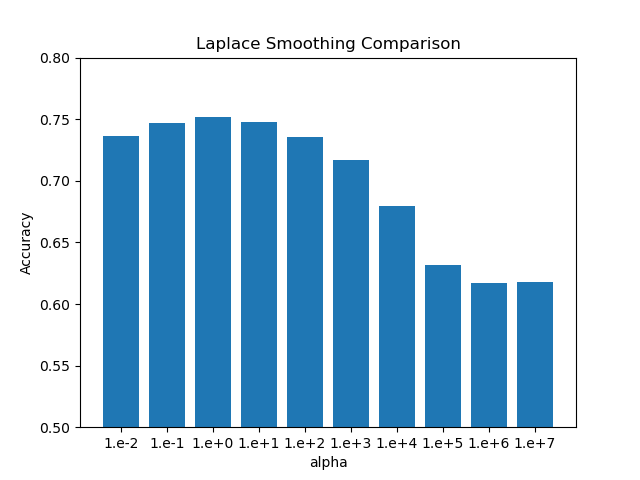
\includegraphics[width=\textwidth,height=\textheight,keepaspectratio]{images/image5.png}
    \caption{Comparació valor Laplace Smooth}
    \label{fig:lap_smooth}
\end{figure}
